\documentclass[10pt,twocolumn]{article}
	
\usepackage{myfontstyle}
\usepackage{mypackages}
\usepackage{mymacros}
\usepackage{mycommands}
\usepackage{graphicx}
\usepackage{hyperref}

\begin{document}
\thispagestyle{fancy1}

%%% Title and Abstract------------------------
\twocolumn[
\begin{center}
	\hrule
	\vspace{3pt}
	% Title:
	{\sffamily\bfseries\Large
		Report for Assignment 9: Tabular Q-Learning for Warehouse Navigation
	} \\
	{\color{gray}
		\vspace{3pt}
		\hrule
		\vspace{3pt}
	}
	{
		\hspace*{\fill}
		Julian Soh
		\hspace*{\fill}
%		Second Author
%		\hspace*{\fill}
%		Third Author
%		\hspace*{\fill}
%		Fourth Author    % uncomment these two lines if there's a fourth author
%		\hspace*{\fill}
	}\\
	\vspace{3pt}
	{\itshape
		\hspace*{\fill}
		Department of Mechanical Engineering, Saint Martin's University
		\hspace*{\fill} \\
		\hspace*{\fill}
		ME/EE 467---Machine Intelligence
		\hspace*{\fill}
	}\\
	\vspace{3pt}
	{
		\hspace*{\fill}
		\today{} % today's date ... can type manually instead
		\hspace*{\fill}
	}
	\vspace{3pt}
	{\color{gray}\hrule}
%	\vspace{2pt}
\end{center}
% Abstract:
\begin{adjustwidth}{1.5in}{1.5in}
{\small
\noindent\textbf{Abstract.} \hspace{1em}
Implement Q-learning and State-Action-Reward-State-Action (SARSA) from scratch for the  warehouse MDP, compare their learned policies to the value iteration solution from Chapter 4, and investigate the effect of exploration schedules and learning rates on convergence.
}
\end{adjustwidth}
\vspace{9pt}
\hrule
\vspace{1\baselineskip}
]

%%% Body -------------------------

\section{Introduction} 
\label{sec:introduction}

This experiment studies \textbf{tabular reinforcement learning} in a small stochastic warehouse navigation problem. The environment is a $4 \times 4$ grid world in which an agent starts at the lower-left corner and must learn how to reach a goal state at $(3, 3)$ while avoiding a hazardous state at $(3, 2)$. The task is intentionally simple enough that the full state space can be represented exactly with a tabular value function, yet rich enough to highlight important reinforcement-learning ideas such as stochastic transitions, exploration, bootstrapping, and the difference between \textbf{off-policy} and \textbf{on-policy} learning.

Beyond comparing reward curves, we also compared the learned policies directly against the optimal policy from value iteration. This makes it possible to identify which states are learned correctly and where the methods differ, particularly in states in close proximity to the hazard.

Overall, this experiment is designed to show not only whether the agent learns successfully, but also \textbf{how different reinforcement-learning algorithms behave under uncertainty}. In particular, it illustrates why Q-learning often learns more aggressive goal-directed behavior, while State-Action-Reward-State-Action (SARSA) can learn safer policies in risky regions because it accounts for the consequences of continued exploration.

\section{Methods}

\subsection{Warehouse and Robot Setup}
The warehouse setup and robot behavior are summarized below:
\begin{itemize}
	\item The warehouse environment is \textbf{stochastic}: the intended action is followed with probability $0.8$, and each perpendicular action occurs with probability $0.1$.
	\item This transition uncertainty requires the robot to plan under risk, rather than follow a deterministic shortest path.
	\item Reward design: each non-terminal transition gives a living reward of $-0.04$.
	\item Terminal rewards: reaching the goal gives $+1$, while entering the hazard gives $-1$.
	\item As a result, the learned policy must balance efficiency (shorter routes) against safety (avoiding hazard-adjacent states).
\end{itemize}

\subsection{Comparing Q-learning vs SARSA}
The main goal of the experiment was to compare \textbf{Q-learning} and \textbf{SARSA} on the same control problem (The Warehouse). Both algorithms learn action values from sampled experience, but they differ in a fundamental way. 

Q-learning uses the greedy backup target $\max_a Q(s', a)$ and therefore learns toward the optimal policy regardless of the exploratory action actually taken. 

SARSA instead updates using the action chosen by the current $\varepsilon$-greedy policy, so it learns the value of behaving according to its current exploration strategy. This distinction is especially important near the hazard, where exploratory mistakes can be costly.

We created the accompanying Jupyter notebook to carry out the following sequence of steps:
\begin{itemize}
	\item Verify required Python packages and imports (NumPy, Matplotlib, and related dependencies).
	\item Implement the warehouse environment class, including stochastic transitions, rewards, terminal states, and reset/step interaction.
	\item Implement $\varepsilon$-greedy action selection and train Q-learning for 1000 episodes.
	\item Extract the Q-learning policy using $\pi(s)=\arg\max_a Q(s,a)$ and summarize training rewards.
	\item Implement and train State-Action-Reward-State-Action (SARSA) for 1000 episodes under the same environment and comparable hyperparameters.
	\item Extract the SARSA policy and compare it to the Q-learning policy qualitatively on the grid.
	\item Compute a value-iteration benchmark to obtain the optimal expected return from the start state.
	\item Plot rolling-average learning curves (window size 50) for Q-learning and SARSA on the same axes, together with the optimal-return reference line.
	\item Compare learned policies against the optimal policy by counting state-wise matches and visualizing all policies with arrow plots.
\end{itemize}

\subsection{Hyperparameter Sensitivity}
The accompanying Jupyter notebook also includes a \textbf{hyperparameter sensitivity study} over learning rate $\alpha$ and exploration decay rate $\rho$ to examine how quickly different configurations converge and which settings are unstable or fail to learn reliably.

\section{Results and Discussion}
\label{sec:results}

\begin{figure}[htb]
	\centering
	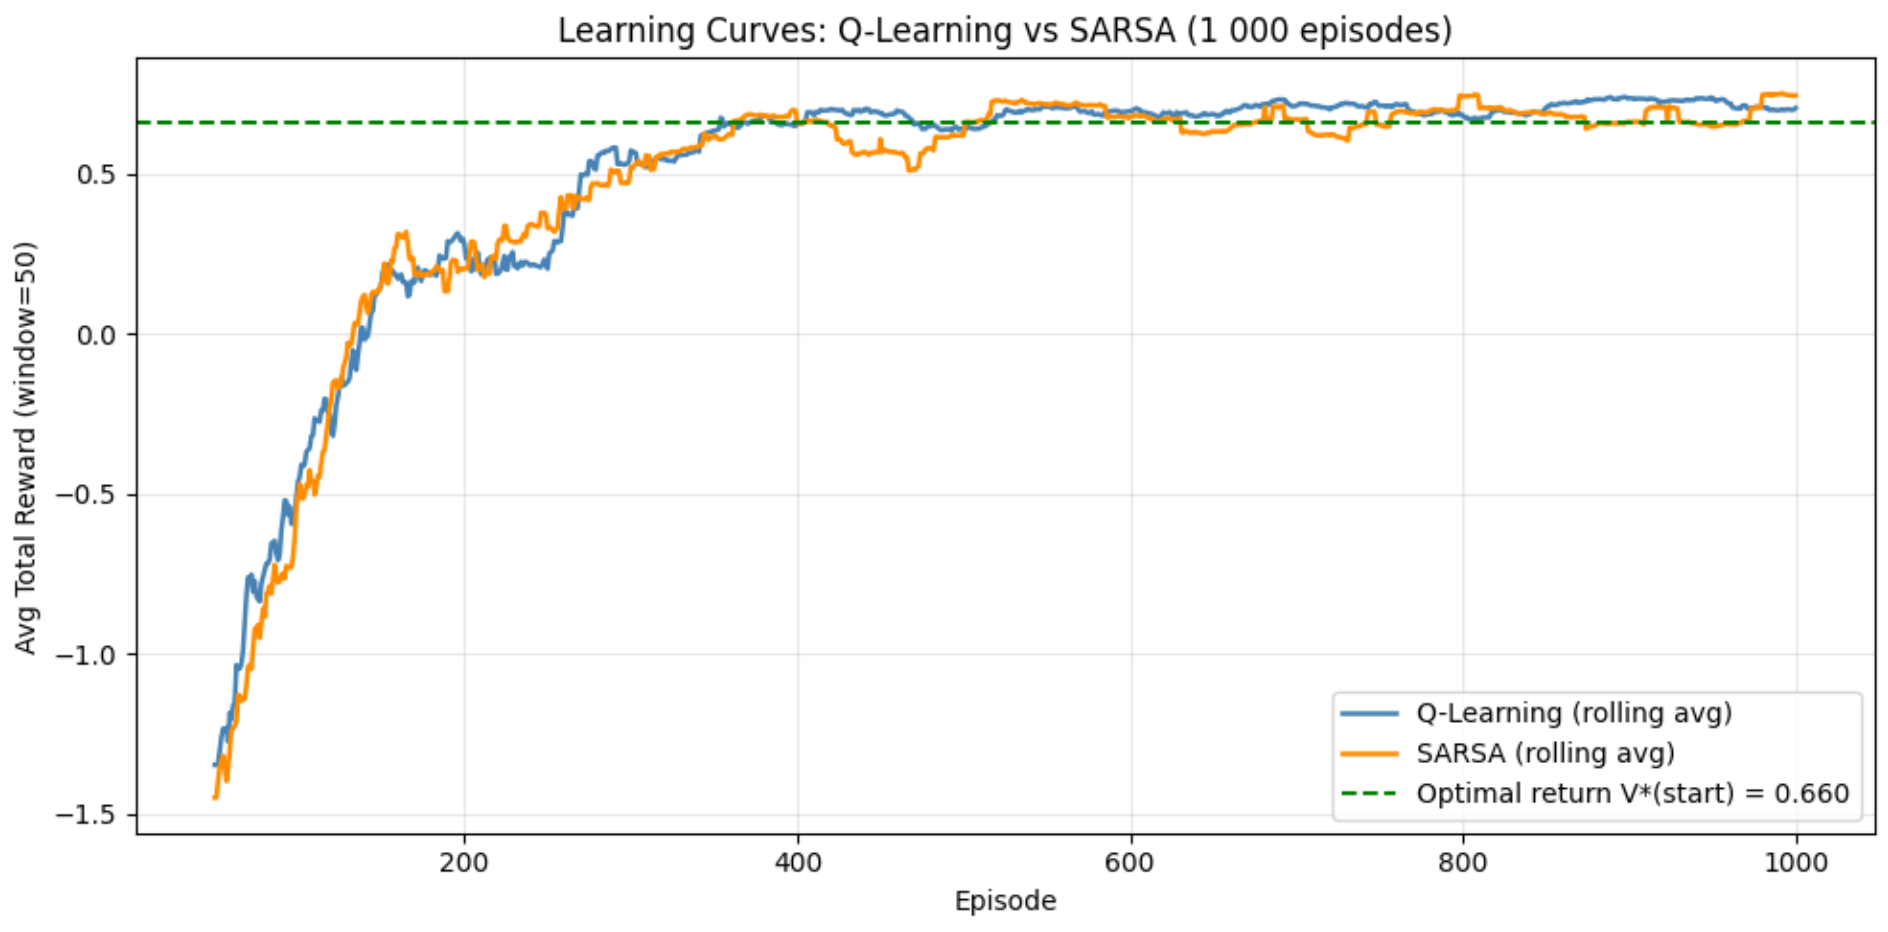
\includegraphics[width=.98\linewidth]{figures/LearningCurves.png}
	\caption{Rolling-average learning curves for Q-learning and SARSA, with optimal-return reference.}
	\label{fig:learning_curves}
\end{figure}

\subsection{Q-Learning}

For Q-learning, the learning-curve behavior in Figure~\ref{fig:learning_curves} shows effective convergence in the tabular setting.

\begin{itemize}
	\item Early training is noisy due to high exploration ($\varepsilon$ near 1), producing wide reward variance and occasional hazard visits.
	\item As $\varepsilon$ decays, returns improve and the learned behavior becomes increasingly consistent and goal-directed.
	\item The reward trend approaches the value-iteration benchmark over training, indicating that the off-policy updates are learning a strong control policy.
\end{itemize}

\subsection{SARSA}

For State-Action-Reward-State-Action (SARSA), Figure~\ref{fig:learning_curves} indicates a stable on-policy learning process with competitive final performance.

\begin{itemize}
	\item Early episodes show high reward variance due to large exploration probability and frequent non-greedy actions.
	\item As $\varepsilon$ decays, returns improve and the learned policy stabilizes, indicating convergence in the tabular setting.
	\item Final performance becomes competitive with Q-learning, while the learning trend is generally smoother during training.
\end{itemize}

\subsection{Policy Comparison}

Figure~\ref{fig:policy_comparison} summarizes the learned-policy behavior and trajectory tendencies for Q-learning and State-Action-Reward-State-Action (SARSA) in the stochastic warehouse grid.

\begin{figure}[htb]
	\centering
	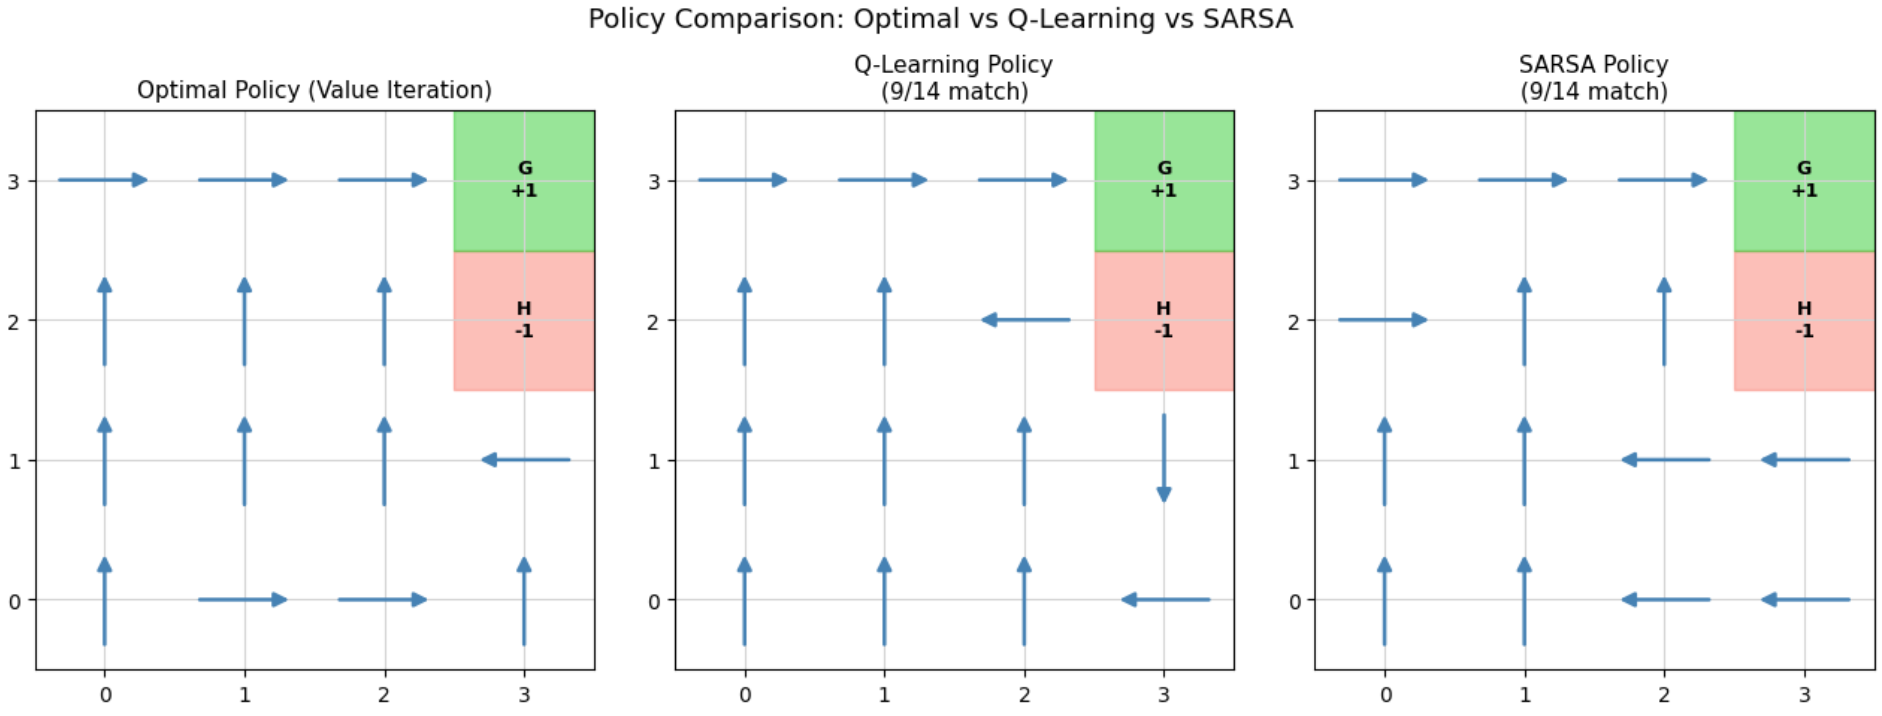
\includegraphics[width=.98\linewidth]{figures/PolicyComparison.png}
	\caption{Policy comparison between Q-learning and SARSA in the warehouse navigation task.}
	\label{fig:policy_comparison}
\end{figure}

\paragraph{Q-learning Policy Behavior}
Q-learning uses the optimistic target $\max_a Q(s',a)$, which tends to favor aggressive action choices in risky regions. In Figure~\ref{fig:policy_comparison}, this appears as a tendency to route closer to the hazard when that path is shorter.

\begin{itemize}
	\item The learned route can prioritize shorter trajectories even when they pass near hazardous states.
	\item Near $(3,2)$, Q-learning is more likely to choose high-reward but higher-risk actions than SARSA.
\end{itemize}

\paragraph{SARSA Policy Behavior}
Because SARSA updates from the action actually taken, it internalizes exploration risk in its value estimates. As shown in Figure~\ref{fig:policy_comparison}, this produces a more conservative policy near the hazard.

\begin{itemize}
	\item SARSA tends to keep a wider safety margin around $(3,2)$ than Q-learning.
	\item The resulting policy is less aggressive but more risk-aware in high-penalty regions.
\end{itemize}

\subsection{Hyperparameter Sensitivity Experiment}

Figure~\ref{fig:hyperparameter_sensitivity} shows the 3\,$\times$\,3 learning-curve grid for Q-learning across learning rates $\alpha \in \{0.01, 0.1, 0.5\}$ and exploration-decay rates $\rho \in \{0.99, 0.995, 0.999\}$.

\begin{figure}[htb]
	\centering
	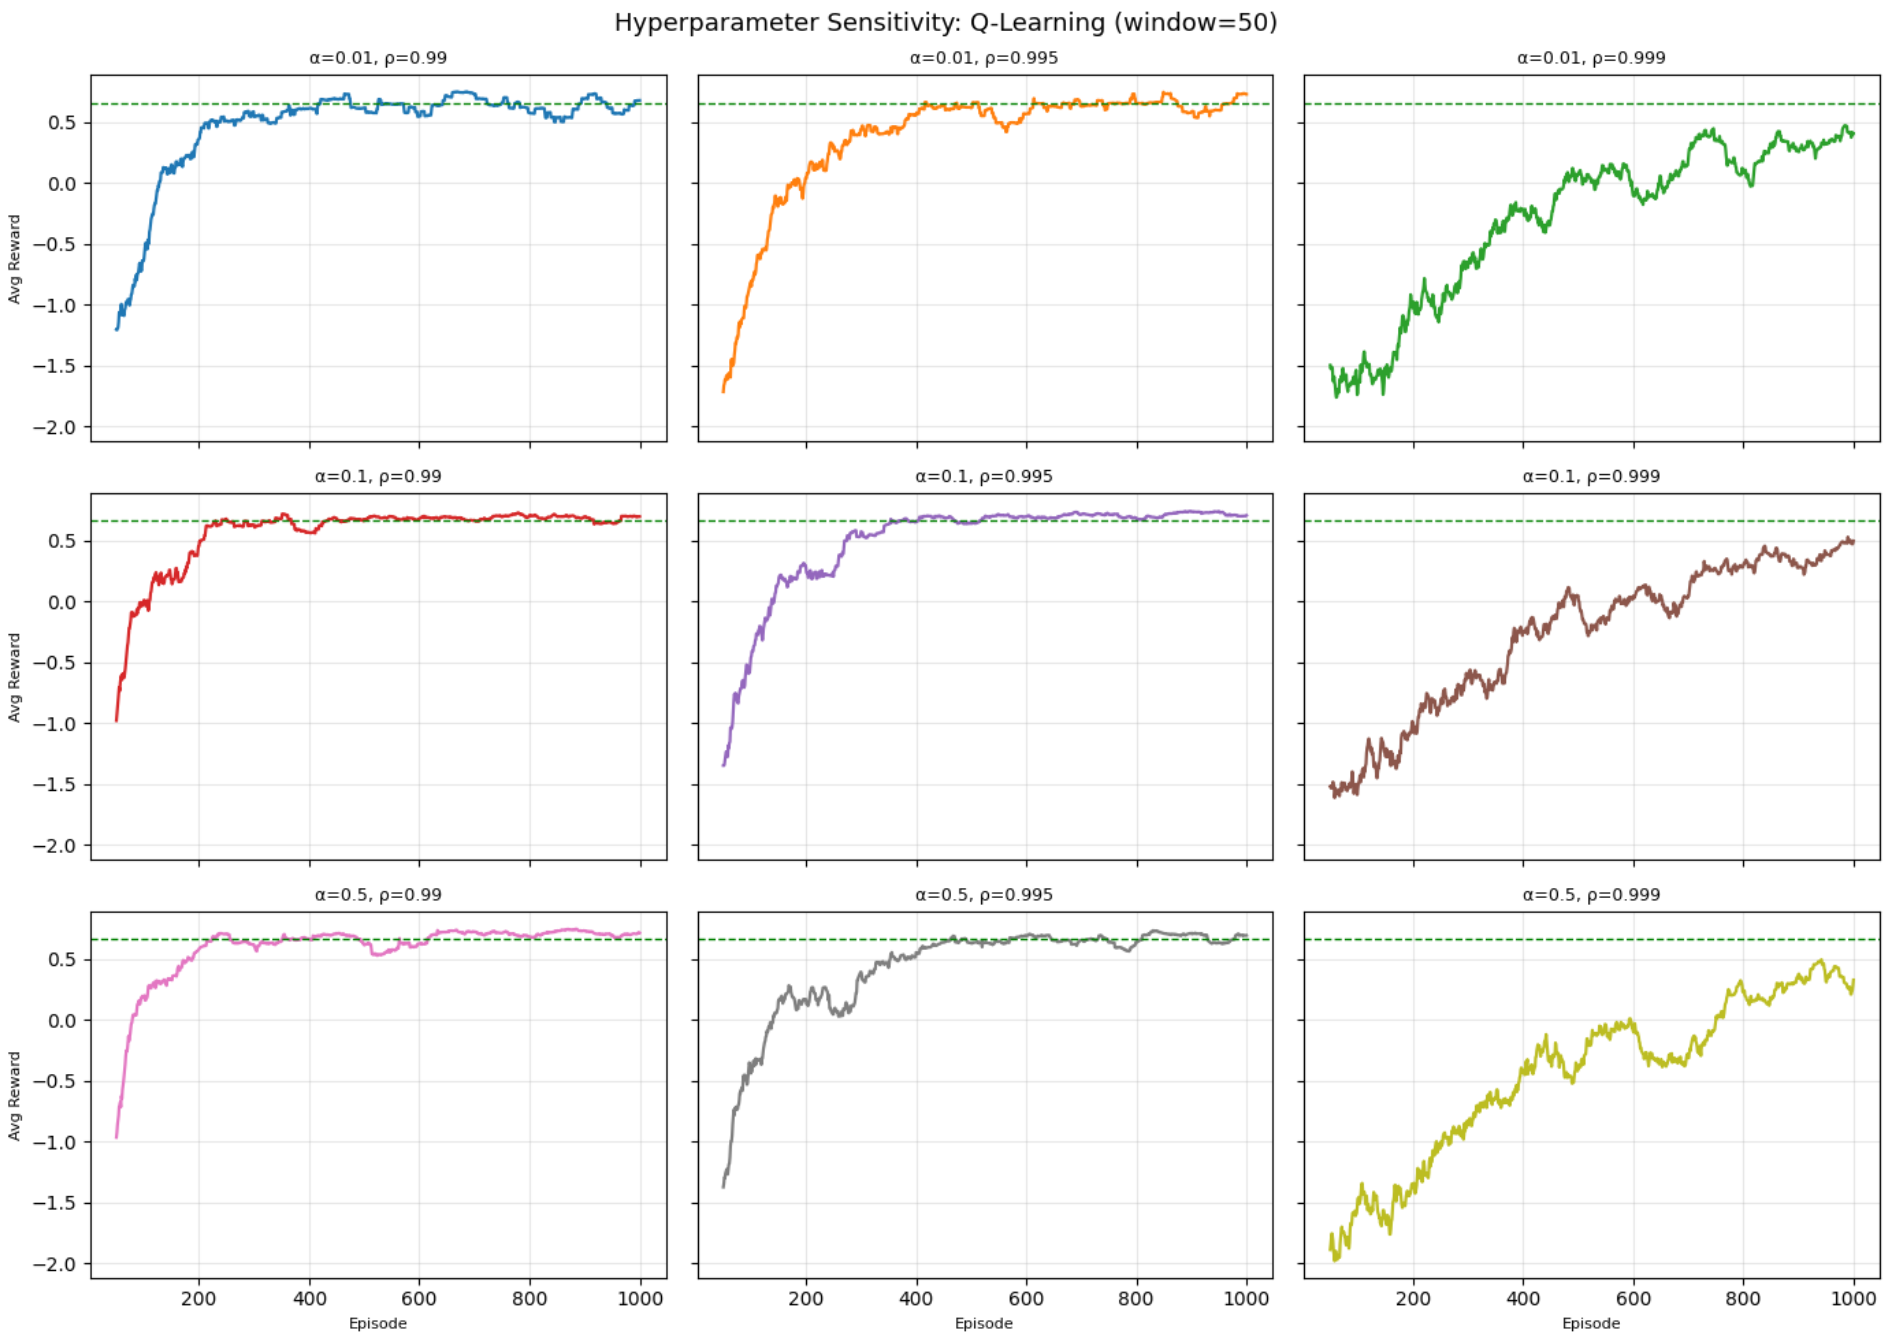
\includegraphics[width=.98\linewidth]{figures/HyperparameterSensitivity.png}
	\caption{Hyperparameter sensitivity for Q-learning across $(\alpha,\rho)$ combinations.}
	\label{fig:hyperparameter_sensitivity}
\end{figure}

From Figure~\ref{fig:hyperparameter_sensitivity}, several trends are clear:

\begin{itemize}
	\item Faster exploration decay ($\rho=0.99$) generally produces the quickest reward improvement across tested learning rates.
	\item Moderate decay ($\rho=0.995$) remains competitive but typically converges slightly later than $\rho=0.99$.
	\item Slow decay ($\rho=0.999$) tends to underperform within 1000 episodes because prolonged exploration delays policy stabilization.
\end{itemize}

The learning-rate effect is also visible in Figure~\ref{fig:hyperparameter_sensitivity}:

\begin{itemize}
	\item $\alpha=0.1$ provides the best balance between convergence speed and stability.
	\item $\alpha=0.5$ can improve quickly for favorable decay settings, but exhibits larger oscillations in some panels.
	\item $\alpha=0.01$ is stable but learns more slowly, especially when paired with $\rho=0.999$.
\end{itemize}

Overall, the best-performing region in this experiment is around $\alpha \in [0.1, 0.5]$ with $\rho \in [0.99, 0.995]$, while configurations with very slow decay are less effective within the fixed training budget.

\section{Conclusion}

This experiment demonstrated that tabular reinforcement learning can learn effective navigation behavior in a stochastic warehouse environment with sparse terminal rewards and a hazard penalty. Both Q-learning and State-Action-Reward-State-Action (SARSA) improved substantially over training and produced policies that were broadly aligned with the value-iteration benchmark. The learning-curve results confirmed that both methods are viable in this domain, with Q-learning often showing faster reward gains, while SARSA displayed smoother adaptation under ongoing exploration.

The policy-level comparison highlighted the key behavioral difference between off-policy and on-policy learning. Q-learning, driven by the $\max_a Q(s',a)$ target, tended to prefer shorter and more aggressive routes, including routes that pass closer to the hazard when they provide higher expected return. In contrast, SARSA internalized exploration risk through its on-policy update and therefore learned more conservative trajectories that maintain a wider safety margin near hazardous states. This distinction is important in practical robotics settings where risk tolerance and safety constraints matter as much as path efficiency.

The hyperparameter sensitivity experiment further showed that convergence quality is strongly dependent on both learning rate and exploration schedule. Faster or moderate exploration decay ($\rho \in [0.99, 0.995]$) produced better performance within the fixed 1000-episode budget than very slow decay ($\rho=0.999$), which kept exploration high for too long. A moderate learning rate ($\alpha=0.1$) provided the most reliable balance between speed and stability, while higher learning rate ($\alpha=0.5$) could converge quickly but with more oscillatory behavior, and lower learning rate ($\alpha=0.01$) converged more slowly.

Overall, the results support three conclusions: (1) both algorithms can learn strong policies in this warehouse MDP, (2) Q-learning is typically more reward-aggressive whereas SARSA is more risk-aware near hazards, and (3) careful hyperparameter selection is essential for stable and efficient convergence.

%%% References -------------------------

\nocite{*}
\bibliographystyle{plainnat}
\bibliography{report}


%%% Appendices -------------------------

\end{document}  